\begin{figure}[htbp]
\begin{center}
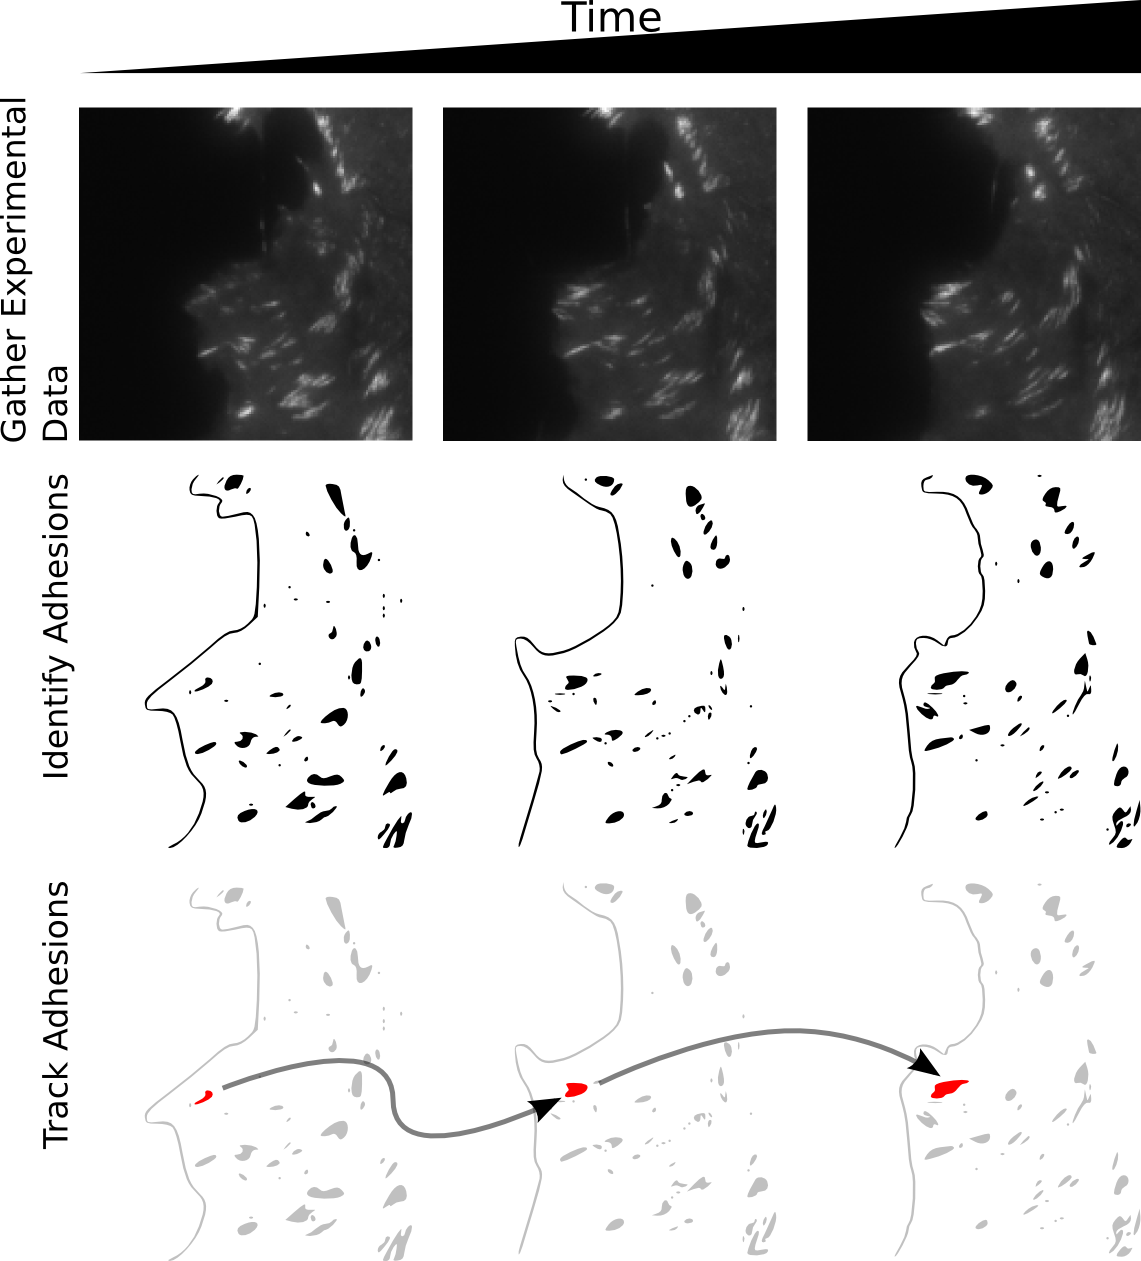
\includegraphics[width=\textwidth]{../figures/FA_workflow/graphic_workflow}
\end{center}
\caption{
{\bf Automating the analysis of focal adhesion images requires a multi-stage
pipeline.} The first row shows several representative example images of
fluorescently labeled Paxillin using TIRF micrscopy. These images only show a
small portion of the entire NIH 3T3 cell imaged in this experiment. In the
second row, a cartoon depiction of the segmented adhesions and the cell edge
are shown. Identification of the adhesions in each image allows a set of static
morphological and fluorescence intensity based features to be extracted. The
third row shows a single adhesion (highlighted in red) being tracked through
the short sample time course. While a single adhesion is highlighted in this
example, all the detected adhesions are tracked though each experiment. The
properties of each adhesion is tracked through time, allowing the large scale
dynamics of the focal adhesions to be determined.  
}
\label{method_flow}
\end{figure}

\begin{figure}[htbp]
\begin{center}
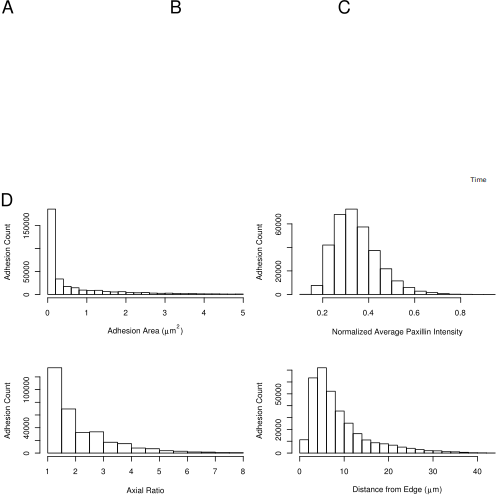
\includegraphics[width=0.8\textwidth]{../figures/statics/statics}
\end{center}
\caption{
{\bf Applying quantitative image processing methods to FA images allows
comprehensive characterization of FA properties.} (A) One frame from a 200
minute movie of NIH 3T3 cells expressing GFP-Paxillin (the scale bar represents
10 $\mu$m). (B) The same cell as in (A), with each adhesion outlined in a
different color. (C) The entire set of adhesions in an experiment can be
visualized by overlaying the adhesions from each microscopy image going from the
first image collected to the last image collected. This example includes the
adhesions from 198 images. (D) A large range of properties can be extracted from
the segmented FA, five samples are provided.  The area histogram was filtered to
only include adhesions with areas less than 5$\mu$m$^2$. The axial ratio
histogram was filtered to only include adhesions with an axial ratio of 8 or
less. The longevity histogram was filtered to include only adhesions with
lifetimes greater than 10, but less than 100 minutes. The histograms include
data from 21 cells.
}
\label{statics}
\end{figure}


\begin{figure}[htbp]
\begin{center}
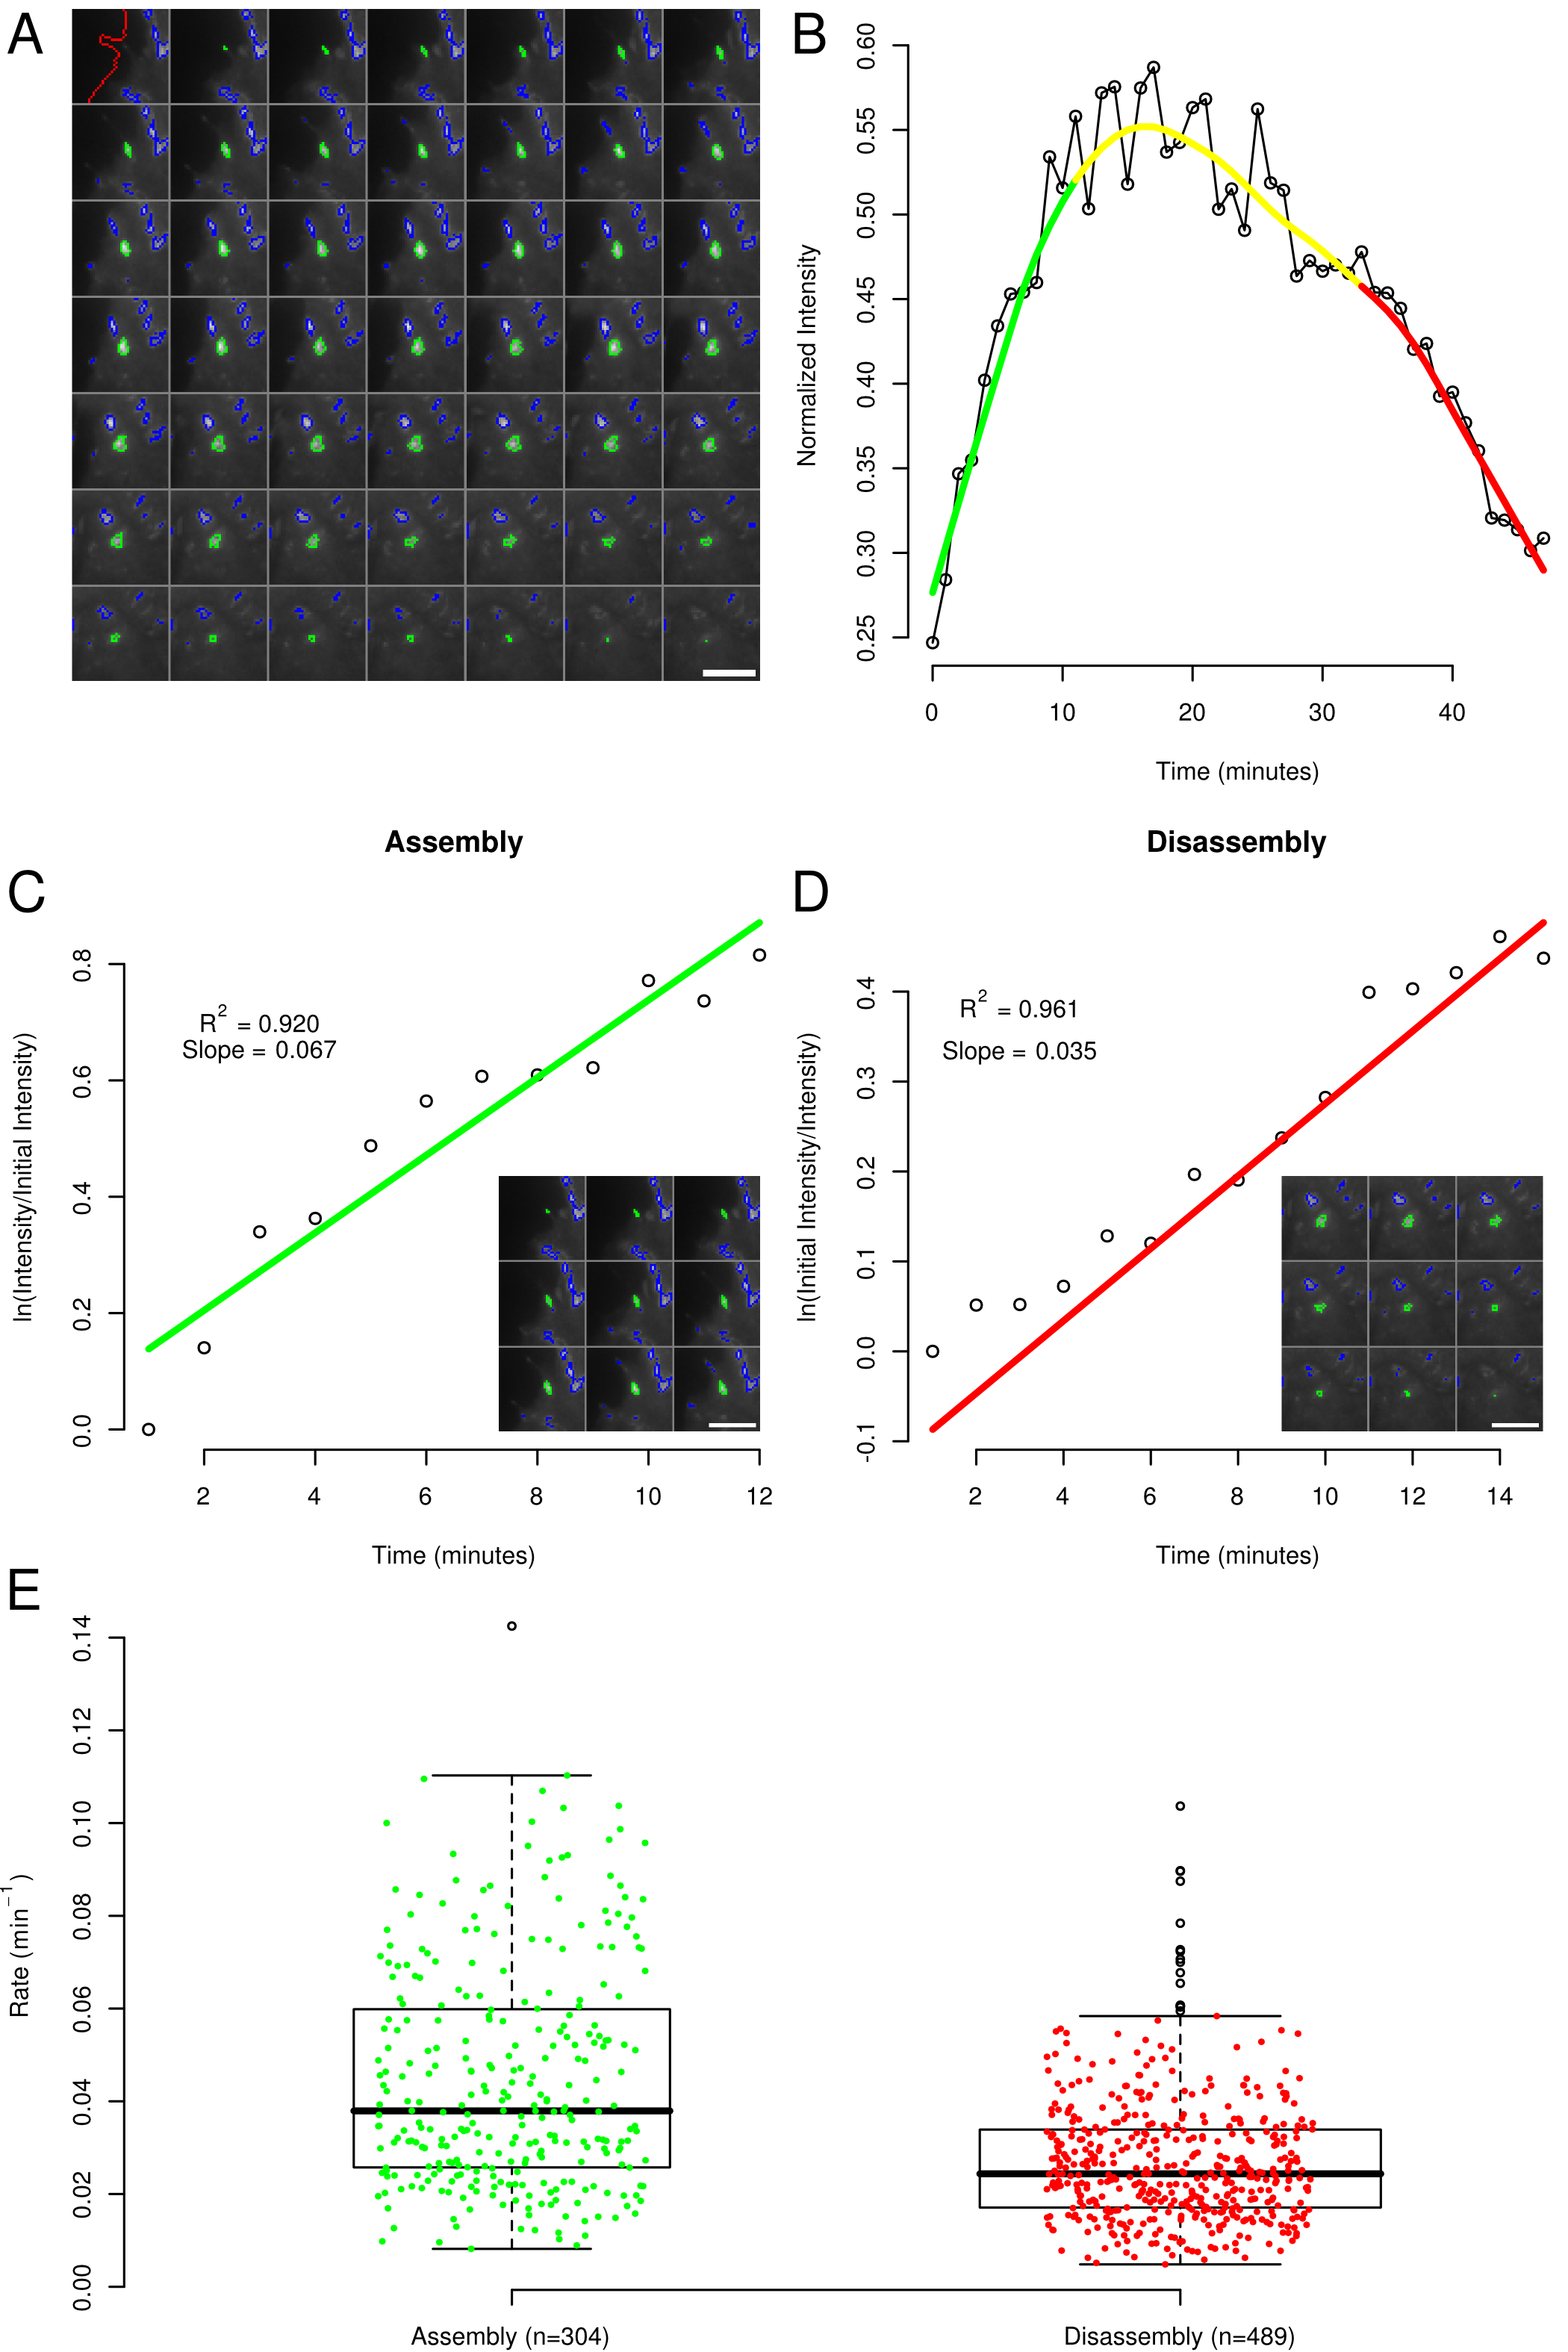
\includegraphics[height=0.8\textheight]{../figures/kinetics/kinetics}
\end{center}
\caption{
{\bf Focal adhesion kinetics.} (A) Each of the adhesions in the cells is
tracked, allowing the position and properties of single adhesions to be
assessed. Here a single adhesion (in green), the surrounding adhesions (in blue)
and the cell edge (in red) are followed for 49 minutes. The cell edge is only
outlined in the first frame. (B) The intensity of the paxillin in the tracked
adhesion in (A) through time. The red line is a smoothed fit to the data using
the lowess algorithm. (C) The normalized log-linear fit of the Paxillin
intensity through time during the assembly phase of the adhesion in part (B).
The inset depicts several of the images from which the Paxillin intensity was
gathered. The color highlights indicate the same cell features as in (A). (D)
The normalized log-linear fit of the Paxillin intensity through time during the
disassembly phase of the adhesion in part (B). The inset depicts several of the
images from which the Paxillin intensity was gathered. The color highlights
indicate the same cell features as in (A). (E) The assembly and disassembly
rates for adhesions whose Paxillin intensity curve fits have R$^2$ values of 0.9
or greater. The scale bar is 10 $\mu$m.
}
\label{kinetics}
\end{figure}

\begin{figure}[htbp]
\begin{center}
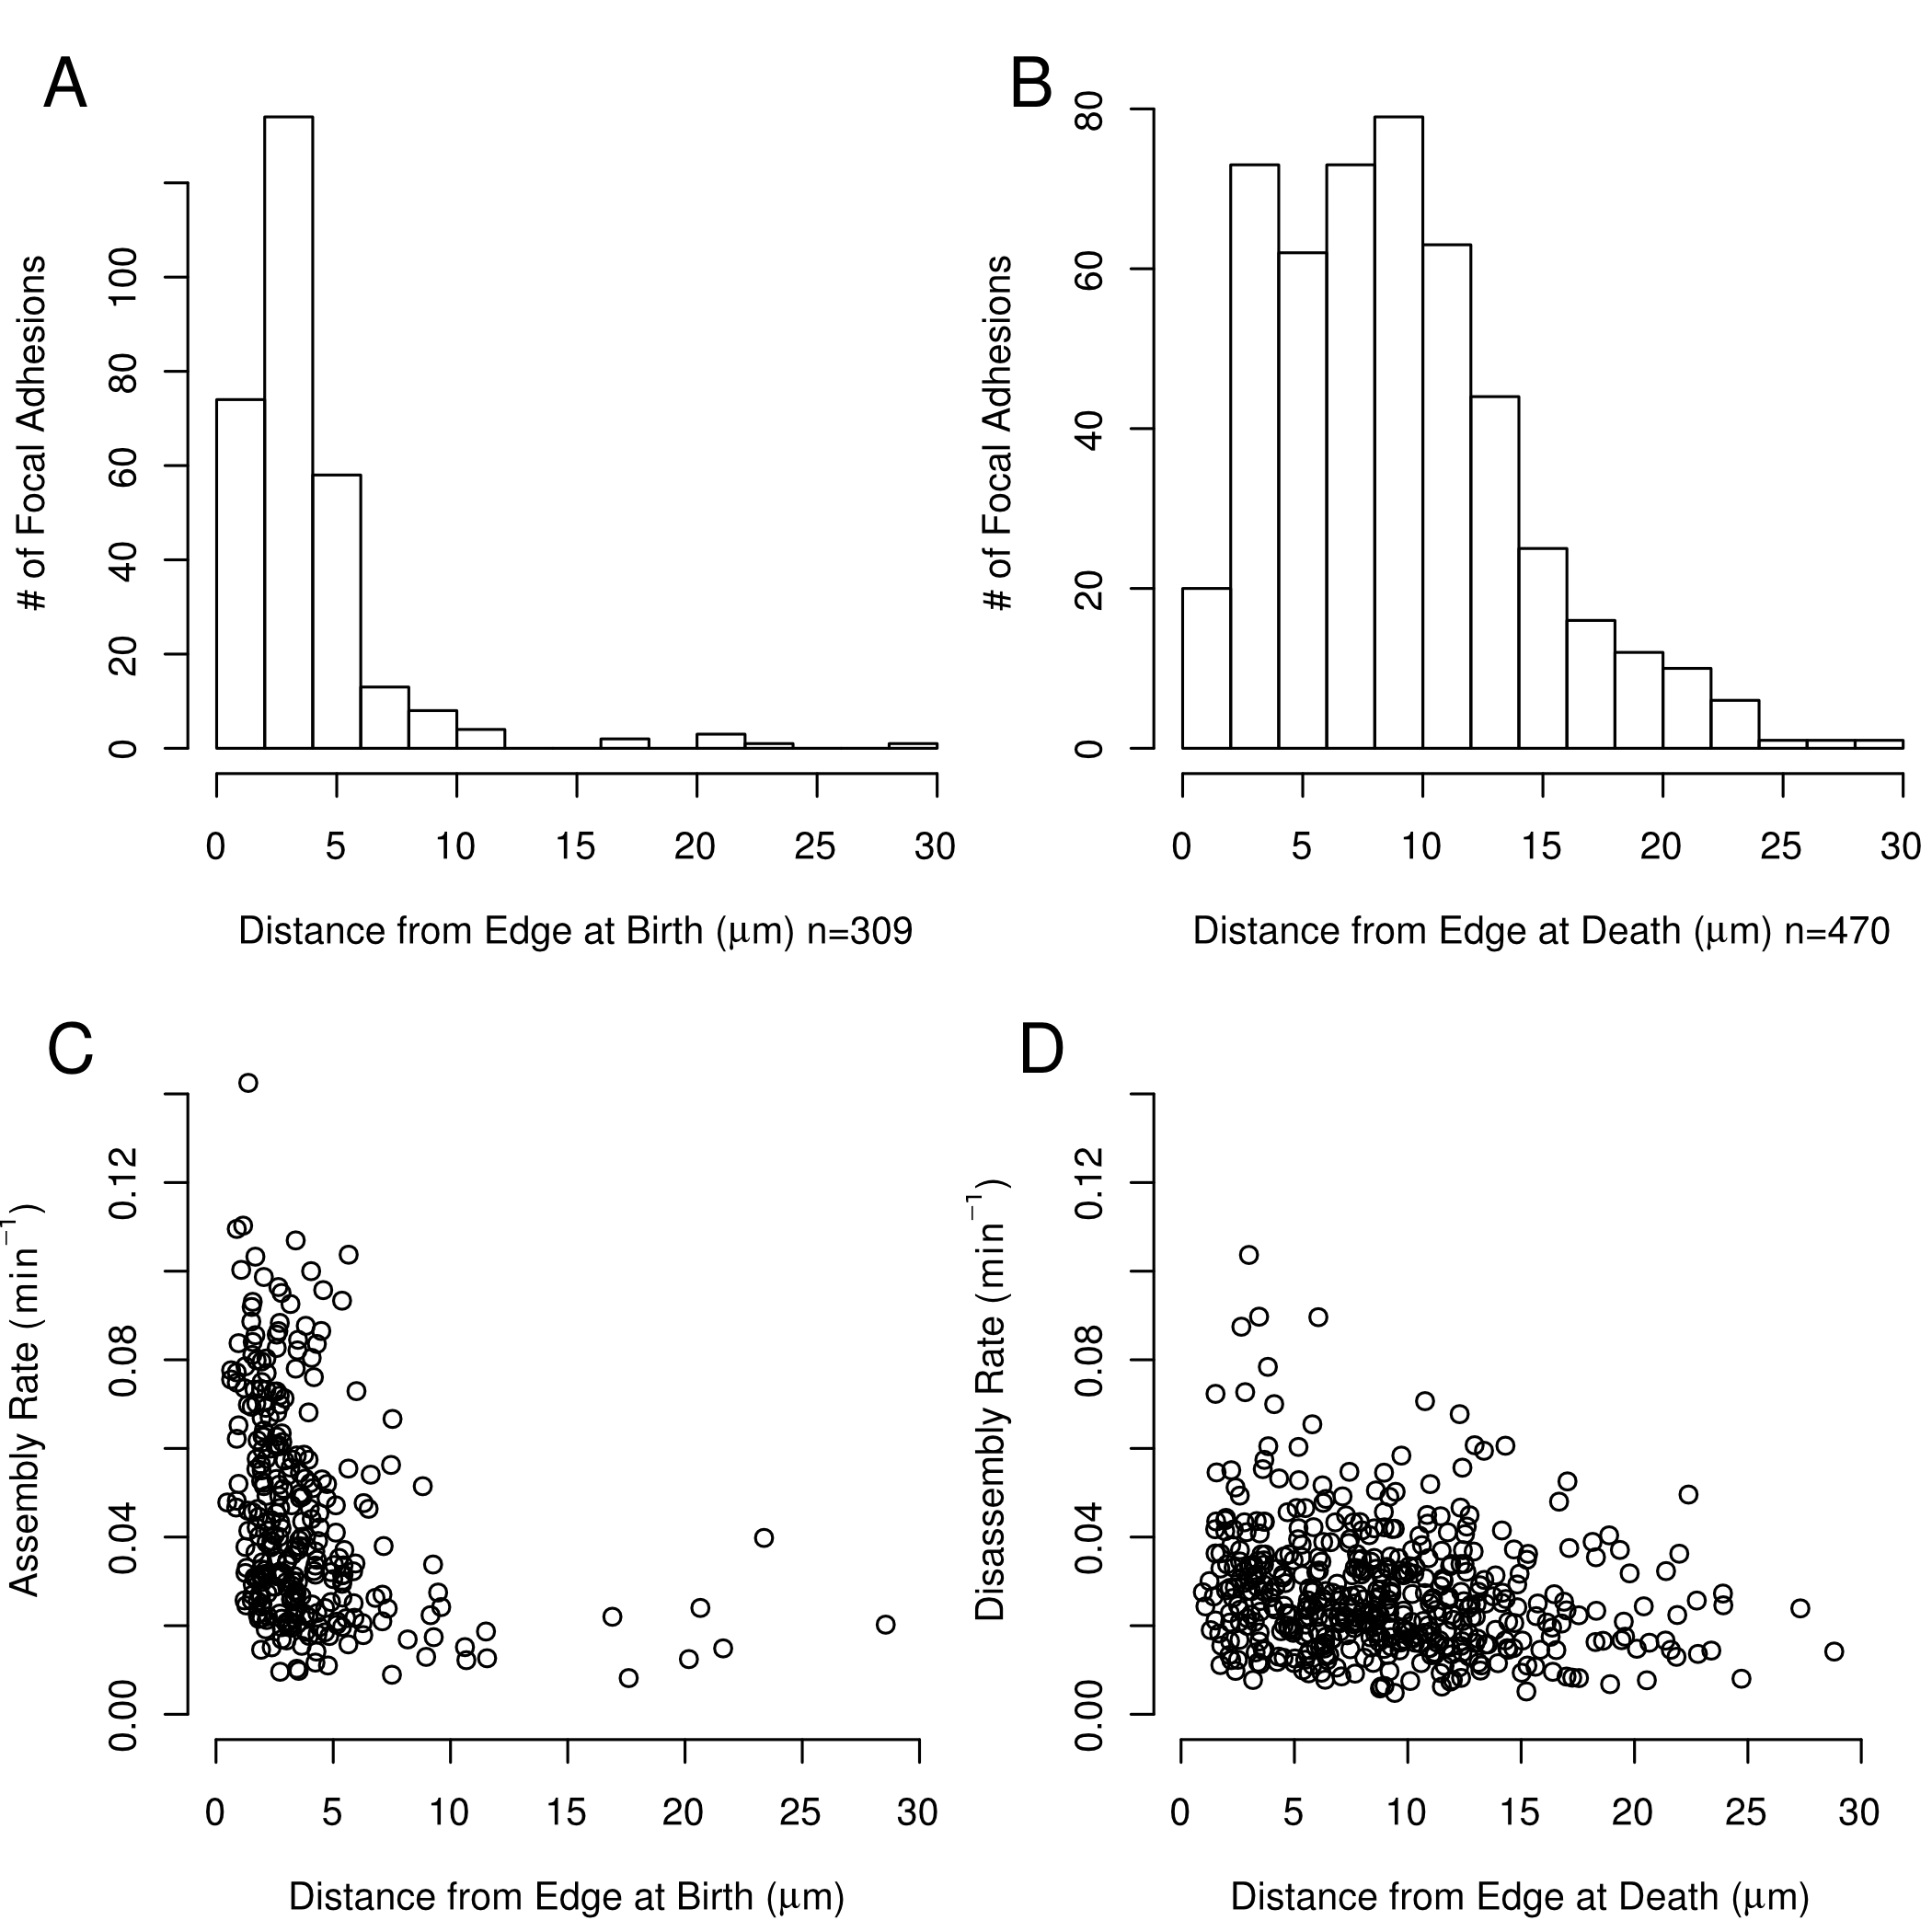
\includegraphics[width=\textwidth]{../figures/spacial/spacial}
\end{center}
\caption{
{\bf Spacial properties of FA centroid positions at birth and death where the
assembly and/or disassembly phases fit a log-linear model with R$^2$ value of
0.9 or greater.} (A) The majority of adhesions whose growth patterns demonstrate
a strong linear model are born within 5 $\mu$m of the cell edge. (B) The
distribution of the distance of death location from the cell edge indicates that
adhesion disassembly typically occurs along a broader band at the cell edge as
compared to the position at adhesion birth. (C) The variance of assembly rates
is greatest for adhesions born within $\sim$5 $\mu$m of the edge (D) The
variance of disassembly rates only has a slight decrease as the distance from
edge at death increases.  
}
\label{spacial}
\end{figure}

\begin{figure}[htbp]
\begin{center}
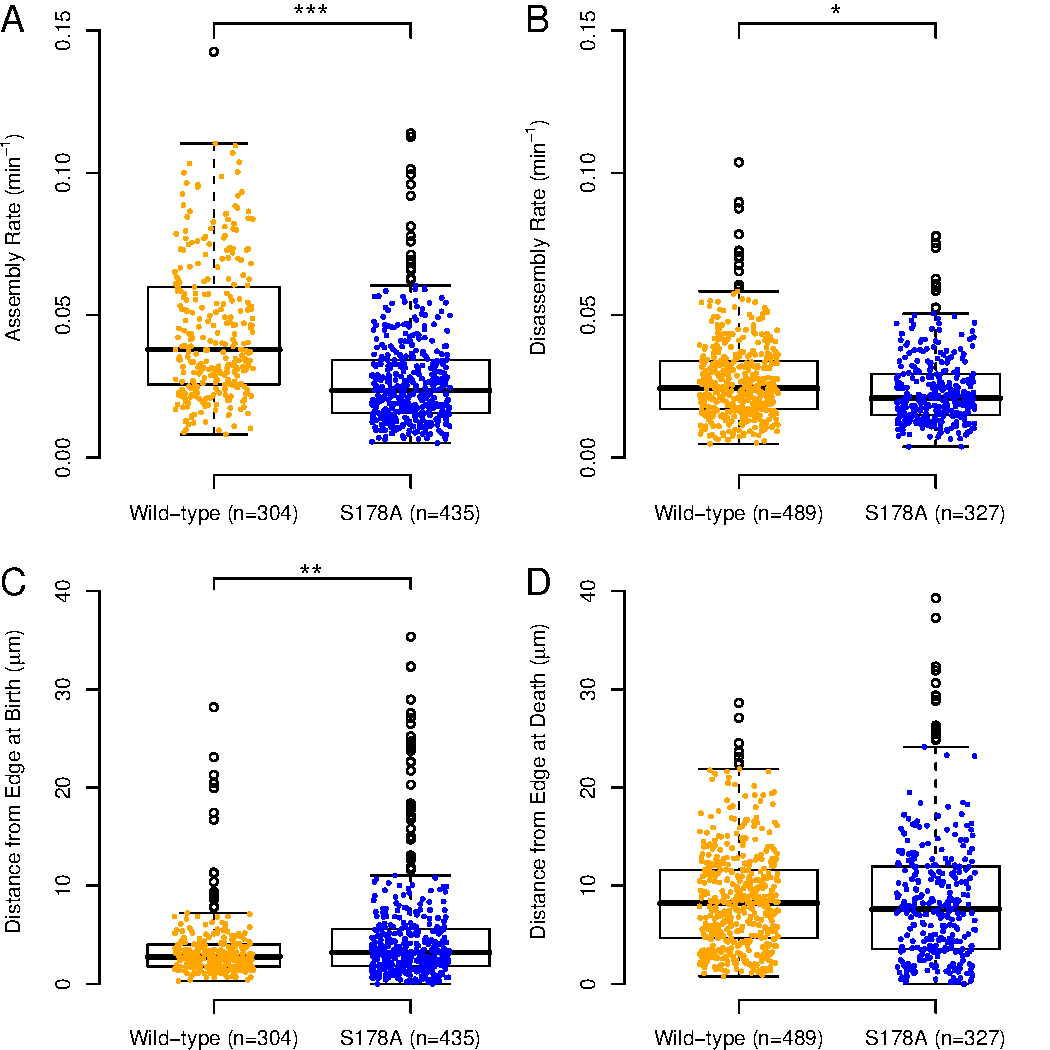
\includegraphics[width=\textwidth]{../figures/S178A/S178A_vs_wild-type}
\end{center}
\caption{
{\bf Comparison between several of the properties of the S178A mutants and
wild-type FA in adhesions which fit a log linear model with R$^2$ value of 0.9
or greater.} (A) The mean assembly rate is decreased by 40\% in the S178A case
(*** indicates $p<10^{-5}$). (B) The mean disassembly rate is also decreased,
but only by 16\% (** indicates $p<10^{-3}$). (C and D) The median position of
adhesion centroids at birth is increased by 44\% (** indicates $p<10^{-3}$),
while the median position of the adhesion centroid at death is unaffected in the
S178A mutants. All p-values were calculated using the bootstrapped
confidence intervals.  }
\label{S178A}
\end{figure}

\begin{figure}[htbp]
\begin{center}
\includegraphics[width=\textwidth]{../figures/lifetimes/adhesion_phase_lifetimes}
\end{center}
\caption{
{\bf The assembly and disassembly phases in S178A mutant FA are significantly
longer than those in the wild-type, while the stability phase lengths are
unaffected.} The phase length values include all adhesions where the log-linear
models fit with a p-value of 0.05 or less.  Error bars indicate 95\% confidence
intervals on the mean phase length as determined through 50,000 bootstrap
samples. A triple asterisk (***) indicates $p<10^{-5}$ and single asterisk (*)
indicates $p<0.05$. Wild-type N Values: Assembly (1057), Stability (456),
Disassembly (1371); S178A N Values: Assembly (2089), Stability (868),
Disassembly (1761)
}
\label{lifetimes}
\end{figure}

\begin{figure}[htbp]
\begin{center}
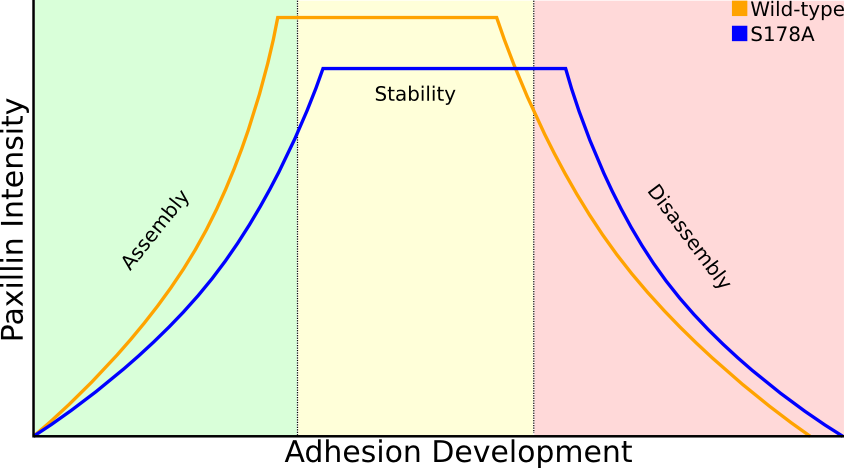
\includegraphics[width=\textwidth]{../figures/S178A/sample_timecourse}
\end{center}
\caption{
{\bf Mutations affecting the interaction of Jun Kinase with Paxillin modify all
stages of FA development.}  }
\label{summary}
\end{figure}
